\chapter{教小孩统计分析} % Introduction chapter suppressed from the table of contents

\hypertarget{ux6559ux5c0fux5b69ux7edfux8ba1ux5206ux6790}{%
\section{教小孩统计分析}\label{ux6559ux5c0fux5b69ux7edfux8ba1ux5206ux6790}}

如果你觉得统计学很高深,可以看看 这个如何教小孩统计分析的故事。

\hypertarget{ux4eceux8003ux8bd5ux6210ux7ee9ux5230ux8d38ux6613ux9006ux5dee}{%
\section{从考试成绩到贸易逆差}\label{ux4eceux8003ux8bd5ux6210ux7ee9ux5230ux8d38ux6613ux9006ux5dee}}

孩子问:爸爸,你是做什么工作的?我明天要在班上介绍自己父母的工作。\\
我:帮客户做统计分析。\\
孩子:统计分析?\\
我心里想你这初中孩子,要如何给你解释统计分析呢?\\
我尝试用一个他可以想象的场景来介绍------假如下面是你班里同学的数学成绩,你会用什么方式把这些成绩表达出来?\\
孩子有点迷茫。\\

\hypertarget{ux4eceux5206ux6790ux5230ux884cux52a8}{%
\subsubsection{20名学生在数学考试中的分数(满分为100分,按大小排序)}\label{ux4eceux5206ux6790ux5230ux884cux52a8}}

30, 35, 37, 40, 40, 49, 51, 54, 54, 55\\
57, 58, 60, 60, 62, 62, 65, 67, 74, 89

我:任何样本数据,都可以用图加平均值、范围等来表达。\\
举例:我们可以画茎叶图(Stem and leaf plot)(详见附件)表达这些学生成绩:\\
%\href{文件:MA_FA2_1.0.1.jpg}{文件:MA FA2 1.0.1.jpg}\\

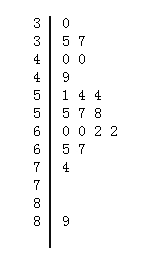
\includegraphics[width=6cm]{MA_FA2_101.jpg}

把20组数从最低排到最高。排在第十位的学生和第十一位的学生的平均数56,叫中位数(Median)。
排第五名和第六名成绩的平均值 44.5,就是Q1四分之一。
排十五名和十六名的平均值 62,就是Q3四分之三。

这个例子中茎叶图再加上Q1、Q2(中位数)、Q3,{[}44.5 , 56 ,
62{]}便可以总括表达这二十个学生的成绩分布。 也可以用下面的柱状图 /
直方图表达:\\
%\href{文件:MA_FA1_1.0.png}{文件:MA FA1 1.0.png}

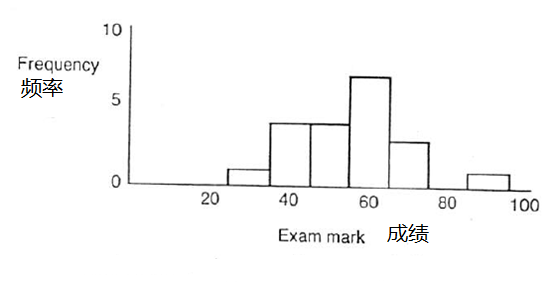
\includegraphics[width=6cm]{MA_FA1_10.png}

也可以利用 Q1、Q2、Q3 (统称四分位数)画箱线图来表达(详见附件)\\
除了中位数,也常用平均值(Mean)来表示一堆数据的中间趋势,平均值就是把所有数据加起来,然后把总数除以数量,比如上面20学生数学成绩的平均值是......\\
孩子充满自信,打断我说:这个平均值简单,我懂。\\
我说:好啊,你这么懂平均值,我问你一个小问题?\\

\framebox{%
\begin{minipage}[t]{0.97\columnwidth}\raggedright
 问题:5、10、350、355
的平均数是多少?
\strut
\end{minipage}}

孩子拿了计算器算出:180。\\
我:你知道那些数是代表什么吗?\\
孩子:不知道。\\
如果这些数是代表角的度数,它的平均值应该是零,而不是
180。这是统计分析很重要的概念------你必须知道那些数的背景,否则你的分析没意义。如果你把那四个数字当成是距离来算均值是
180,与四个角度数求均值的结果就完全不一样了。\\
从以上例子,你就知道了解问题背景(Context)很重要。

孩子:这些统计分析有什么用?\\
我:例如有了这成绩的分析,你就可以知道自己的成绩在整个班是处于什么位置?也可以帮你比较不同科目的成绩。

\hypertarget{ux6bd4ux8f83ux4e09ux79cdux6559ux5b66ux65b9ux6cd5}{%
\subsubsection{比较三种教学方法}\label{ux6bd4ux8f83ux4e09ux79cdux6559ux5b66ux65b9ux6cd5}}

45名学生被随机分成5个大小相同的组。两组(A、B)采用目前使用的方法(控制组),另外三组(C、D、E)采用三种新方法。实验结束时,所有学生参加了一次标准测试,结果(满分30分)见表B.1。关于教学方法的差异,可以得出什么结论?\\
B.1

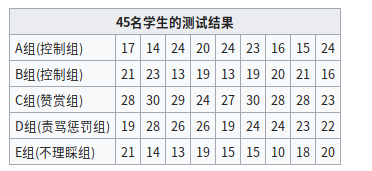
\includegraphics[width=6cm]{Screenshotfrom2023-11-0920-08-48.png}

我:你可以用刚学过的四分位数(Q1、Q2、Q3)配合箱线图表示每一组数据分布,然后看看有没有差异。这样你便可以比较五个班的成绩。\\
他过了十五分钟就画了五个组的箱线图:\\
%\href{文件:图片61-3.1.jpg}{500px}

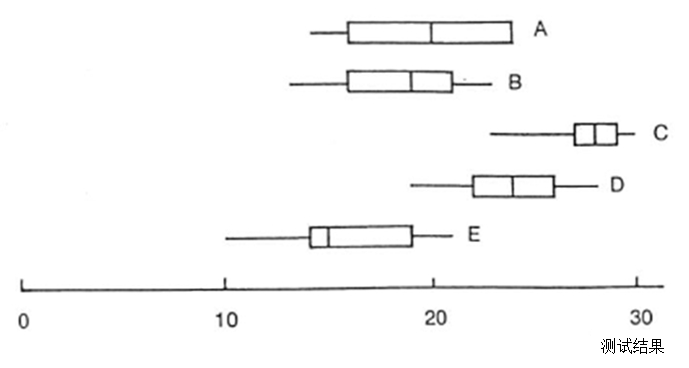
\includegraphics[width=6cm]{图片61-31.jpg}

我:能看到显著区分吗?\\
孩子:看得出是C组最好,D组也比较好,E组就比较差。\\
我:是的,但如果我们只是比较5个组成绩的平均值,没有考虑每一班成绩范围,便不能全面比较。例如:上面数学考试成绩的Q1
Q2 Q3是(44.5 、 56 、62)如果C组的数学成绩是(32 、57.5 、63)
你会认为C组比你们好吗?虽然中位数比你们班高,但Q1比你们低很多,所以不能单看中位数(或平均值)比较。

看到他对这些挺有兴趣,我便问他如何表达以下数据:\\

\hypertarget{ux4ebaux4e00ux5e74ux5185ux9605ux8bfbux6708ux520aux7684ux6570ux91cf}{%
\subsubsection{20人一年内阅读月刊的数量}\label{ux4ebaux4e00ux5e74ux5185ux9605ux8bfbux6708ux520aux7684ux6570ux91cf}}

0, 1, 11, 0, 0, 0, 2, 12, 0, 0\\
12, 1, 0, 0, 0, 0, 12, 0, 11, 0

我看他开始使用同样方法,
我便说这些统计数据跟前面学生成绩的分布不一样,它一头一尾最高,这表示大部分人要么就是不看杂志,要么就是每个月都看,这种分布就不合适用刚才那些方法去表达,只能说它有两个高峰,或者叫众数(mode),再配上一个柱状图。如果我们用中位数或者这些数的平均值,或三分位数来表达的话,反而是误导读者,不能正确的表达那些数据的分布。\\
%\href{文件:MA_FA4_1.0.png}{文件:MA FA4 1.0.png}\\

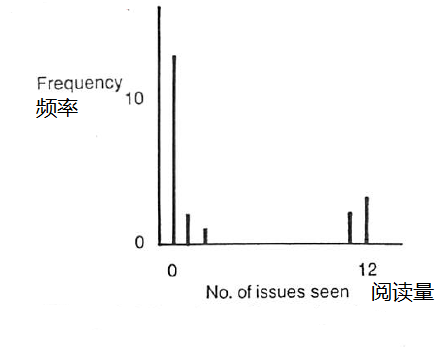
\includegraphics[width=6cm]{MA_FA4_10.png}

当总体(population)包含非常多数据时,就只能抽样,用抽样来估计population分布。但是要注意,如果样本不是随机抽样(random
sample),可能会导致出来的参数偏离、产生误差。\\
我看孩子一头雾水,但我记得他很喜欢研究二战的战斗机,我就用下面这个例子说明,这样抽样出来的结论是没有意义。\\

\hypertarget{ux53d6ux6837ux504fux5dee-survivors-bias}{%
\subsubsection{取样偏差 Survivor's
Bias}\label{ux53d6ux6837ux504fux5dee-survivors-bias}}

错误的抽样会导致错误结论。

\framebox{%
\begin{minipage}[t]{0.97\columnwidth}\raggedright
二战时会对那些没有被击落的战斗机,研究哪个部分被德军的攻击最多,针对这些部位去加强防护,希望增高飞机的存活率。你同意吗?我们只是抽样了未被击落的飞机,被击落的都未被抽样。一个比较正确的抽样是所有两类都抽样才比较合理。\\ 
其实被击落的飞机哪个部分被击中更重要,但是我们无法得到那些抽样,只可以从没有被击落的飞机去看,这是抽样的错误。所以分析得出的结论没有意义。\\
%\href{文件:WW2Screenshot_2021-04-07_222054.1.jpg}{600px}}}

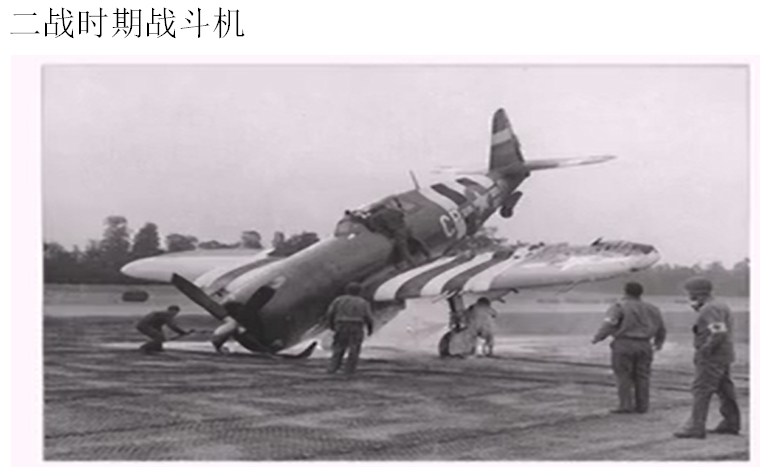
\includegraphics[width=6cm]{WW2Screenshot_2021-04-07_2220541.jpg}
\strut
\end{minipage}}

我:你看看下面例子,便会更了解随机抽样的重要性:

\framebox{%
\begin{minipage}[t]{0.97\columnwidth}\raggedright
只挑选合"味道"的来作比较 (Picking
cherries)\\
%\href{文件:儿童MA.1.jpg}{400px}}\\
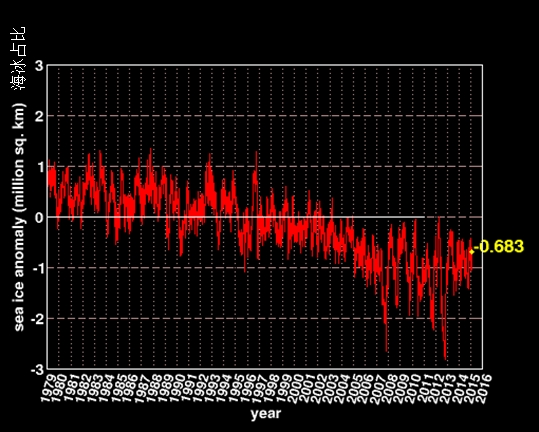
\includegraphics[width=6cm]{儿童MA1.jpg}\\
从上面八零年代到现在全球海洋冰量的统计很明显看到地球在不断地暖软化。但你还可以抽两个时间,例如:2012年四月份的冰量比1988年六月份多,来说明``全球变冷''!
\strut
\end{minipage}}

孩子对统计分析好像越来越感兴趣。\\
我:现在你开始知道什么叫统计了吗?明天可以跟老师讲故事了吗?\\
孩子追着问:可不可以再给我一个练习题?我觉得这统计学也没什么困难,我还可以把你给我的那些题目拿给我同桌小李试试,看他懂不懂(男孩总是要当英雄,出风头)。\\
我:好啊。下面的身高统计数据,请你用刚才的方式来汇总一下,看看你学会没有?\\

\hypertarget{ux540dux5987ux5973ux53c2ux52a0ux67d0ux79cdux75beux75c5ux7814ux7a76ux5979ux4eecux7684ux8eabux9ad8ux4ee5ux7c73ux8ba1ux5206ux522bux4e3a}{%
\subsubsection{20名妇女参加某种疾病研究,她们的身高(以米计)分别为:}\label{ux540dux5987ux5973ux53c2ux52a0ux67d0ux79cdux75beux75c5ux7814ux7a76ux5979ux4eecux7684ux8eabux9ad8ux4ee5ux7c73ux8ba1ux5206ux522bux4e3a}}

1.52, 1.60, 1.57, 1.52, 1.60, 1.75, 1.73, 1.63, 1.55, 1.63\\
1.65, 1.55, 1.65, 1.60, 1.68, 2.50, 1.52, 1.65, 1.60, 1.65

他便拿着纸,用刚才学过的方式计算中位数、三分系数等,蛮有自信地画图、交卷。\\
我:你认识2.5米高的女性吗?\\
小孩:真的好像没有。\\
我:所以里面的2.50
肯定是不对。你为什么没有疑问,直接去做?统计分析必须要判断数据是否正确、是否合理。\\
如果数据本身不可靠,那么怎么分析都没用,我们称之为``垃圾进,垃圾出(Garbage
in, garbage out)。\\
我:也有很多人利用图表误导读者,所以我们看一些统计专家的统计数据分析时也要小心。\\

\hypertarget{ux7f8eux56fdux4e2dux897fux90e8ux623fux4ef7ux8d8bux52bfux56fe}{%
\subsubsection{美国中西部房价趋势图}\label{ux7f8eux56fdux4e2dux897fux90e8ux623fux4ef7ux8d8bux52bfux56fe}}

%\href{文件:Stat_f22-1_1.2.jpg}{500px}

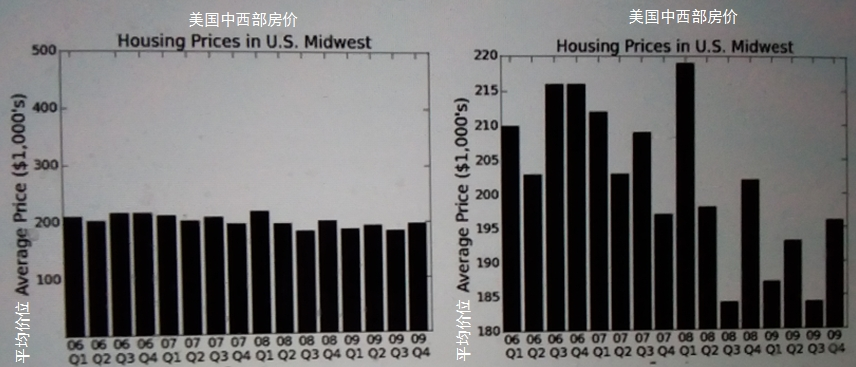
\includegraphics[width=6cm]{Stat_f22-1_12.jpg}

上图是06年到09年每个季度,美国中西部的房价。如果我们看右面那个柱状图,你会认为房价波动很大。但是如果同样这组数据看左面柱状图的话,你就会觉得没有太多变化。所以我们要注意看左面坐标有没有标明数字。不应该仅仅看图。\\
虽然数据都一样,但如图形不一样,传达的信息便完全不同。\\
孩子:你说的我都懂,很简单。\\
我:用统计分析骗人的故事可多。你不是说要今年暑假找暑期工赚钱,下面是一个去工厂找工作的故事:\\
\{\textbar{} class="wikitable" \textbar{}-
\textbar{}小李刚中学毕业,希望去工厂找工作。\\
问:工厂员工薪水是多少?\\
人事部经理面带笑容地跟他说:我们工厂员工平均月收入大概3300。\\
小李进了工厂后,才发现绝大部分的工人月薪是2000。
有多年经验的工人才可以拿到2400。但他们有少数的管理层,他们的平均月薪是25,000。

%\href{文件:AverageSalaryScreenshot_2021-07-31_171502.1.jpg}{400px}

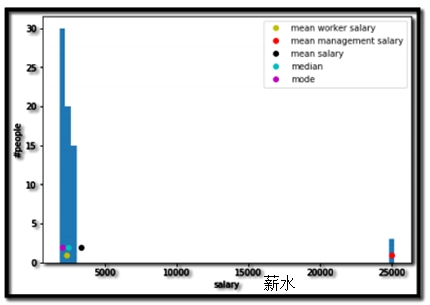
\includegraphics[width=6cm]{AverageSalaryScreenshot_2021-07-31_1715021.jpg}

所以人事部经理没有``骗''小李,工厂员工平均收入是每月3309。

\textbar{}\}

\hypertarget{ux5206ux6790ux4f8bux5b50ux8fdeux7eedux4e0eux5206ux7ec4ux6570ux636e}{%
\section{分析例子:连续与分组数据}\label{ux5206ux6790ux4f8bux5b50ux8fdeux7eedux4e0eux5206ux7ec4ux6570ux636e}}

第二天,孩子乖乖地来找我,他说:爸爸,今天我跟老师说了你的工作是做统计分析,老师听到就发我一些高年级的生物实验数据,希望帮他做些分析,看两类实验有没有差异。你可以帮忙吗?\\

\hypertarget{ux8695ux8c46ux690dux7269---ux53ccux6837ux672ctux68c0ux9a8c}{%
\subsubsection{蚕豆植物 -
双样本T检验}\label{ux8695ux8c46ux690dux7269---ux53ccux6837ux672ctux68c0ux9a8c}}

以下数据比较10个剪枝和10个生根样本中某一化学物质的浓度:\\
剪枝:53, 58, 48, 18, 55, 42, 50, 47, 51, 45\\
生根:36, 33, 40, 43, 25, 38, 41, 46, 34, 29\\
~\\
我:你可以同样用昨天学过的方法(如,柱状图)比较两组数。\\
孩子就按这个汇总了两个实验数据的分布。\\
%\url{文件:图片61-1.1.png}

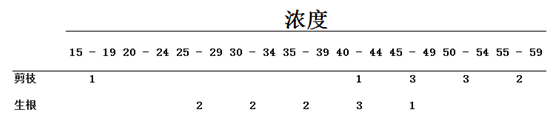
\includegraphics[width=6cm]{图片61-11.png}

我:你应该也看出:剪枝样本有一个很明显的异常点------18。你应该问老师,18是否错误还是值得相信的数?如果18是不对,你就很明显看到上面剪枝的平均浓度比下面生根高。如果不能``看''出来就可以用``双样本T''检验比较两组数据是否有显著差异。但是如果有刚刚那种异常点,如直接用双样本
T
分析,因为第一组数据被那个18拉低了,得出结果是两组没有显著差异。所以还是直接看数据的分布更实在。

我:我们在统计学可以使用假设检验(注),其中包括双样本T检验比较,方差分析(ANOVA)等,就是针对这类统计数据分析。但是在你这个实验数据,从画图一眼都能看出有显著区分,就不需要再采用假设检验,因采用那些方法不会得出额外的信息。\\
我接着跟他说:有些时候统计数据不是连续数据,像学生成绩、浓度、高度等,而是分组数据。例如下面这些国外人种眼睛颜色与头发颜色的数据,这种数据我们就需要用列联表
(Contingency Table) 来识别这两个变量之间有没有关系。\\

\hypertarget{ux5934ux53d1ux548cux773cux775bux989cux8272ux7684ux4e0dux540cux7ec4ux5408}{%
\subsubsection{头发和眼睛颜色的不同组合}\label{ux5934ux53d1ux548cux773cux775bux989cux8272ux7684ux4e0dux540cux7ec4ux5408}}

592人的头发和眼睛颜色的不同组合:

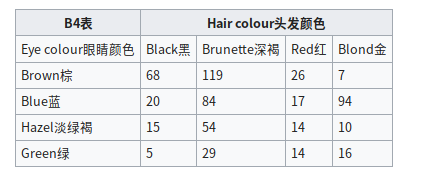
\includegraphics[width=6cm]{Screenshotfrom2023-11-0920-19-09.png}

如果我们利用 B4
表的数,把它那些每一行、每一列进行求和,我们可以看见每列或者每行的分析结果。例如棕色(brown)眼睛的占大多数,但金发
(blond)例外,金发的大部分是蓝(blue)眼睛。其实也看到金头发的那列跟其他的一些分布很不一样。比如我们看每行的话,也可以看到棕色眼睛跟蓝眼睛的数量差不多。但在金头发(blond)和黑头发(black)的列分布就不一样了。统计分析的卡方检验也可以帮我们分析分组数据间有没有相关。但刚才这类简单4×4
数据表,计算出B7列联表便足够,卡方检验没有带来更多有用信息。\\
\textbf{实际(Obs.) 数量表}:

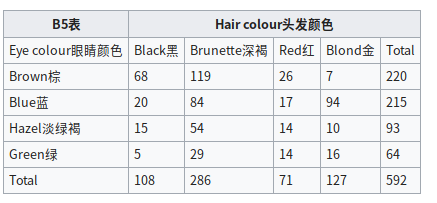
\includegraphics[width=6cm]{Screenshotfrom2023-11-0920-20-47.png}

\textbf{实际(Obs.) vs 预计(Exp.)数量表 Contingency Table}:

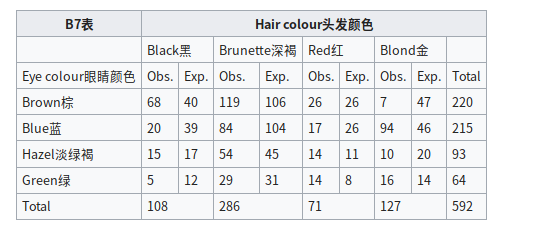
\includegraphics[width=6cm]{Screenshotfrom2023-11-0920-21-37.png}

\begin{description}
\item[]
\begin{description}
\tightlist
\item[]
注:双样本T检验,方差分析(ANOVA),卡方检验等都属于假设检验,下一章会详细介绍各种假设检验方法。
\end{description}
\end{description}

\hypertarget{ux603bux7ed3}{%
\section{总结}\label{ux603bux7ed3}}

统计分析主要是希望利用数据分析、统计方式帮我们解决问题(Problem
Solving),所以度量的重点是如何分析,帮助解决问题。\\
按目标策划收集哪些数据?如何收集?如何分析?

我们也应按以上思路,协助开发团队,更好地利用数据解决问题。

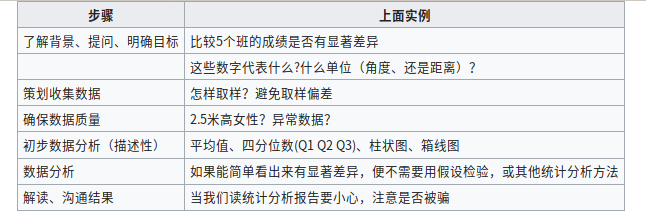
\includegraphics[width=6cm]{Screenshotfrom2023-11-0920-22-37.png}

\hypertarget{ux9644ux4ef6}{%
\section{附件}\label{ux9644ux4ef6}}

\hypertarget{ux5982ux4f55ux753bux830eux53f6ux56festem-and-leaf-plot}{%
\subsection{如何画茎叶图(Stem and leaf
plot)}\label{ux5982ux4f55ux753bux830eux53f6ux56festem-and-leaf-plot}}

以文中20名学生在数学考试分数为例:

\begin{enumerate}
\tightlist
\item
  把分数从小到大排序。
\item
  从上而下画一直线。
\item
  第一个数30,左边写3,右面写0(叶)。
\item
  排第二是35,因5大于0-4,新一行,左边写 3,右面写5(叶)。
\item
  37, 因7属于5\textasciitilde{}9 ,所以同一行,在5右面写7(叶)。
\item
  最终便可以简单利用数目字形成一个横放的直方图。
\end{enumerate}

\hypertarget{ux7bb1ux7ebfux56fe-box-and-whisker-plot}{%
\subsection{箱线图 (Box and Whisker
Plot)}\label{ux7bb1ux7ebfux56fe-box-and-whisker-plot}}

%\href{文件:BoxWhiskerScreenshot_2021-08-02_214603.1.jpg}{500px}

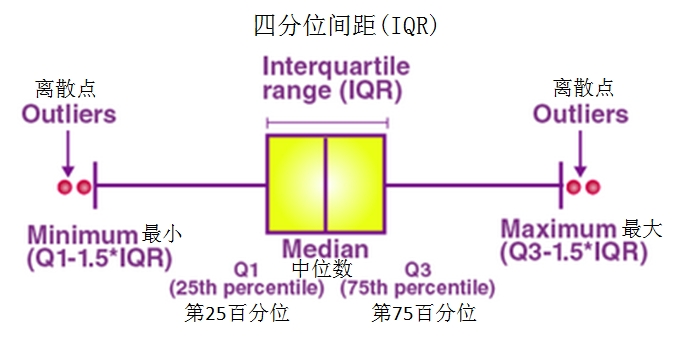
\includegraphics[width=6cm]{BoxWhiskerScreenshot_2021-08-02_2146031.jpg}

箱线图包括5个数:

\begin{itemize}
\tightlist
\item
  Minimum 最少 (Q0 )
\item
  1st Quartile (Q1 , 25 percentile) 箱子的左面边线
\item
  Medium 中位数 (Q2 , 50 percentile) 箱子中间的线
\item
  3rd Quartile (Q3 , 75 percentile) 箱子的右面边线
\item
  Maximum 最大 (Q4 , 100 percentile)
\end{itemize}

有些箱线图直接把两头指到最大与最少,不展示离散点 (outliers)。

Interquartile range (IQR) = Q3 - Q1

\hypertarget{ux53c2ux8003references}{%
\section{参考References}\label{ux53c2ux8003references}}

1. GUTTAG, John V.: "Introduction to computation and programming using
Python" MIT Press 2021\\
2. CHATFIELD, Chris : "Problem Solving: a statistician's guide 2/e"
Chapman \& Hall 1995\\
3. BLUMAN: Elementary Statistics 10/e\\


